\twocolumn[\colorsection{Campo eléctrico de cargas puntuales}]
\setcounter{figure}{0}

\begin{Exercise}
  Una carga puntual de $\SI{-8.0}{\nano\coulomb}$ se localiza en el origen de un sistema de coordenadas. Obtenga el vector campo eléctrico en la posición $\va*{r} = \SI{1.2}{\metre}\vu{i} - \SI{1.6}{\metre}\vu{j}$.
\end{Exercise}
\begin{Answer}
  $\va*{E} = \SI{-10.8}{\newton/\coulomb}\vu{i} + \SI{14.4}{\newton/\coulomb}\vu{j}$
\end{Answer}
%
\begin{Exercise}
Una partícula $\alpha$ es el núcleo de un átomo de helio, que tiene una masa de $\SI{6.64E-27}{\kilogram}$ y una carga eléctrica de $\SI{3.20E-19}{\coulomb}$. Compare la fuerza de la repulsión eléctrica entre dos partículas $\alpha$ con la fuerza de atracción gravitatoria que hay entre ellas, calculando el cociente $F_e/F_g$.
\end{Exercise}
\begin{Answer}
  $F_e/F_g = 3.1\times 10^{35}$
\end{Answer}
%
\begin{Exercise}
Dos cargas puntuales se localizan en el eje $+x$ de un sistema de coordenadas. La carga $q_1 = \SI{1.0}{\nano\coulomb}$ está a $\SI{2.0}{\centi\metre}$ del origen, y la carga $q_2 = \SI{-3.0}{\nano\coulomb}$ está a $\SI{4.0}{\centi\metre}$ del origen. ¿Cuál es la fuerza total que ejercen estas dos cargas sobre una carga $q_3 = \SI{5.0}{\nano\coulomb}$ que se encuentra en el origen?
\end{Exercise}
\begin{Answer}
  $\va*{F} = \SI{-2.8E-5}{\newton}\vu{i}$
\end{Answer}
%
\begin{Exercise}\label{p:puntuales01}
  Tres cargas puntuales, $q_1$, $q_2$ y $q_3$, están equiespaciadas a lo largo de una recta horizontal, como muestra la figura \ref{f:puntuales01}. Si $q_1 = Q$ y $q_2 = -Q$, ¿cuánto deberá valer $q_3$ para que la fuerza neta sobre $q_1$ sea cero?
\end{Exercise}
\begin{Answer}
  $q_3 = 4Q$
\end{Answer}
%
\begin{center}
  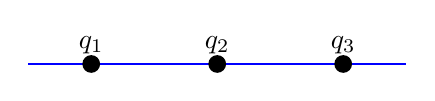
\begin{tikzpicture}[scale=0.8]
    \draw [blue] (0,0)--(6,0);
    \fill [black](1,0) circle(4pt) node[above] {$q_1$};
    \fill [black](3,0) circle(4pt) node[above] {$q_2$};
    \fill [black](5,0) circle(4pt) node[above] {$q_3$};
  \end{tikzpicture}
  \captionof{figure}{Problema \ref{p:puntuales01}\label{f:puntuales01}}
\end{center}
%
\begin{Exercise}
  Tres cargas puntuales están alineadas a lo largo del eje $x$. La carga $q_1 = \SI{3.00}{\micro\coulomb}$ está en el origen, la carga $q_2 = \SI{-5.00}{\micro\coulomb}$ se encuentra en $x = \SI{0.200}{\metre}$, y la tercera carga es $q_3 = \SI{-8.00}{\micro\coulomb}$. ¿Dónde está situada $q_3$ si la fuerza neta sobre $q_1$ es $\SI{7.00}{\newton}$ en la dirección negativa del eje $x$?
\end{Exercise}
\begin{Answer}
  $x = \SI{-0.144}{\metre}$
\end{Answer}
%
\begin{Exercise}
  Considerar la siguiente distribución de cargas: $q_1 = \SI{1}{\milli\coulomb}$ en la posición $\va*{r}_1 = (\SI{0}{\metre};\SI{0}{\metre})$; $q_2 = \SI{3}{\milli\coulomb}$ en la posición $\va*{r}_2 = (\SI{2}{\metre};\SI{0}{\metre})$ y $q_3 = \SI{-2}{\milli\coulomb}$ en la posición $\va*{r}_3 = (\SI{0}{\metre};\SI{1}{\metre})$. Calcular el módulo y el ángulo de la fuerza $\va*{F}_1$ que la distribución ejerce sobre la carga $q_1$.
\end{Exercise}
\begin{Answer}
  \begin{minipage}[t]{.5\textwidth}
    $|\va*{F}_1| = \SI{19.2}{\kilo\newton}$\\ $\theta = \SI{110.6}{\degree}$
  \end{minipage}
\end{Answer}
%
\begin{Exercise}
  Se tienen cuatro cargas puntuales idénticas, de carga $q$, ubicadas en los vértices de un cuadrado de $\SI{20}{\centi\metre}$ de lado. \textit{a}) Calcular la fuerza que sentirá una carga puntual $2q$ situada en el centro del cuadrado. \textit{b}) Calcular la fuerza que actúa sobre esa carga central cuando se quita una de las cargas de los vértices.
\end{Exercise}
\begin{Answer}
  \begin{minipage}[t]{.5\textwidth}
    \textit{a}) $F = 0$\\ \textit{b}) $F = 100kq^2\si{\metre^{-2}}$
  \end{minipage}
\end{Answer}
%
\begin{Exercise}\label{p:puntuales02}
  Dos pequeñas esferas igualmente cargadas y de la misma masa están suspendidas de un mismo punto por dos hilos no conductores de igual longitud $l = \SI{15}{\centi\metre}$, como se muestra en la figura \ref{f:puntuales02}. Debido a la repulsión, el equilibrio se establece cuando las dos esferas están separadas una distancia $d = \SI{10}{\centi\metre}$. Calcular la carga $q$ de cada esfera si la masa de cada esfera es $m = \SI{0.5}{\gram}$.
\end{Exercise}
\begin{Answer}
  $|q| = \SI{44}{\nano\coulomb}$
\end{Answer}
%
\begin{center}
  \begin{tikzpicture}[scale=0.2]
    \draw [blue] (0,0)--(6,0);
    \draw [blue] (0,0)--(0.5,1);
    \draw [blue] (0.5,0)--(1,1);
    \draw [blue] (1,0)--(1.5,1);
    \draw [blue] (1.5,0)--(2,1);
    \draw [blue] (2,0)--(2.5,1);
    \draw [blue] (2.5,0)--(3,1);
    \draw [blue] (3,0)--(3.5,1);
    \draw [blue] (3.5,0)--(4,1);
    \draw [blue] (4,0)--(4.5,1);
    \draw [blue] (4.5,0)--(5,1);
    \draw [blue] (5,0)--(5.5,1);
    \draw [blue] (5.5,0)--(6,1);
    \draw [blue] (3,0)--(-2,-14.14) node[black,midway,left] {$l$};
    \fill [black](-2,-14.14) circle(10pt) node[left] {$q$};
    \draw [blue] (3,0)--(8,-14.14) node[black, midway,right] {$l$};
    \fill [black](8,-14.14) circle(10pt) node[right] {$q$};
    \draw [black, {Stealth}-{Stealth}] (-2,-15)--(8,-15) node[black,midway,above] {$d$};
  \end{tikzpicture}
  \captionof{figure}{Problema \ref{p:puntuales02}\label{f:puntuales02}}
\end{center}
%
\begin{Exercise}\label{p:puntuales03}
Las cargas $q_1 = \SI{2}{\micro\coulomb}$, $q_2 = \SI{-8}{\micro\coulomb}$ y $q_3 = \SI{12}{\micro\coulomb}$ se colocan en los vértices de un triángulo equilátero, cuyos lados miden $\SI{10}{\centi\metre}$, como se muestra en la figura \ref{f:puntuales03}. \textit{a}) Hallar el campo eléctrico en el punto $P$. \textit{b}) Hallar la fuerza sobre una carga de $\SI{-1}{\micro\coulomb}$ si es colocada en $P$.
\end{Exercise}
\begin{Answer}
  \begin{minipage}[t]{.4\textwidth}
    \textit{a}) $\va*{E} = ( -36\vu{i} + 9.6\vu{j} )\times 10^6 \si{\newton/\coulomb}$\\ \textit{b}) $\va*{F} = ( 36\vu{i} - 9,6\vu{j} )\si{\newton}$
  \end{minipage}
\end{Answer}
%
\begin{center}
  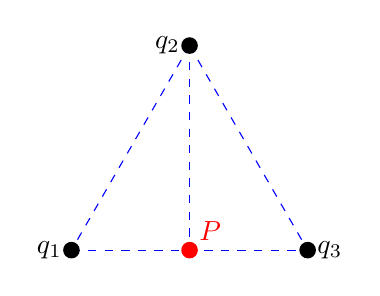
\begin{tikzpicture}[scale=0.3]
    \draw [blue, dashed] (0,0)--(-5,-8.66);
    \draw [blue, dashed] (0,0)--(5,-8.66);
    \draw [blue, dashed] (-5,-8.66)--(5,-8.66);
    \draw [blue, dashed] (0,0)--(0,-8.66);
    \fill [black](-5,-8.66) circle(10pt) node[left] {$q_1$};
    \fill [black](0,0) circle(10pt) node[left] {$q_2$};
    \fill [black](5,-8.66) circle(10pt) node[right] {$q_3$};
    \fill [red](0,-8.66) circle(10pt) node[above right] {$P$};
  \end{tikzpicture}
  \captionof{figure}{Problema \ref{p:puntuales03}\label{f:puntuales03}}
\end{center}
%
\begin{Exercise}\label{p:puntuales04}
  Calcule el módulo del campo eléctrico resultante en el centro de un cuadrado de lado $b$, en cuyos vértices se sitúan las cargas $q$, $2q$, $-4q$ y $2q$, como se muestra en la figura \ref{f:puntuales04}.
\end{Exercise}
\begin{Answer}
  $|\va*{E}| = 10kq/b^2$
\end{Answer}
%
\begin{center}
  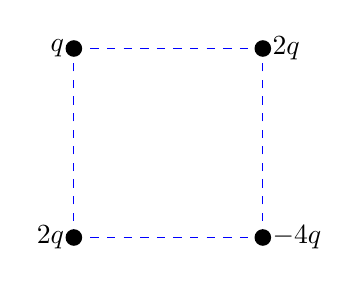
\begin{tikzpicture}[scale=0.6]
    \draw [blue, dashed] (0,0)--(4,0);
    \draw [blue, dashed] (0,0)--(0,4);
    \draw [blue, dashed] (0,4)--(4,4);
    \draw [blue, dashed] (4,0)--(4,4);
    \fill [black](0,0) circle(5pt) node[left] {$2q$};
    \fill [black](0,4) circle(5pt) node[left] {$q$};
    \fill [black](4,0) circle(5pt) node[right] {$-4q$};
    \fill [black](4,4) circle(5pt) node[right] {$2q$};
  \end{tikzpicture}
  \captionof{figure}{Problema \ref{p:puntuales04}\label{f:puntuales04}}
\end{center}
%
\begin{Exercise}\label{p:puntuales05}
  Dos cargas se colocan como se muestra en la figura \ref{f:puntuales05}. La carga $q_1$ vale $\SI{3.00}{\milli\coulomb}$ y se desconocen el signo y el valor de la carga $q_2$. El campo eléctrico neto en el punto $P$ está por completo en la dirección horizontal hacia la derecha, como se observa en la figura. Calcular el módulo del vector campo eléctrico en el punto $P$.
\end{Exercise}
\begin{Answer}
  $|\va*{E}| = \SI{2.8E10}{\newton/\coulomb}$
\end{Answer}
%
\begin{center}
  \begin{tikzpicture}[scale=0.5]
    \draw [blue, dashed] (0,0)--(13,0) node[black, midway,below] {$\SI{13}{\centi\metre}$};
    \draw [blue, dashed] (0,0)--(1.923,4.615) node[black, midway,above left] {$\SI{5}{\centi\metre}$};
    \draw [blue, dashed] (13,0)--(1.923,4.615) node[black, midway,above right] {$\SI{12}{\centi\metre}$};
    \fill [black](0,0) circle(6pt) node[left] {$q_1$};
    \fill [black](13,0) circle(6pt) node[right] {$q_2$};
    \fill [red](1.923,4.615) circle(6pt) node[black, above left] {$P$};
    \draw [red,-{Stealth}, thick] (1.923,4.615)--(8,4.615) node[black, midway,above] {$\va*{E}$};
  \end{tikzpicture}
  \captionof{figure}{Problema \ref{p:puntuales05}\label{f:puntuales05}}
\end{center}
%
\begin{Exercise}\label{p:puntuales06}
  Sobre el eje $x$ se ubican una carga positiva $q$ en la posición $x = d/2$ y una carga negativa $-q$ en la posición $x = -d/2$, como se observa en la figura \ref{f:puntuales06}. De esta forma se tiene un dipolo eléctrico de separación $d$, cuyo momento dipolar es $\va*{p}=qd\vu{x}$, paralelo al eje $x$. Este dipolo se encuentra en una región donde existe un campo eléctrico uniforme que forma un ángulo de $30^\circ$ con el eje $x$. \textit{a}) ¿Cuál es la fuerza neta que ejerce el campo externo sobre el dipolo? \textit{b}) Calcular el torque que siente este dipolo ($\va*{\tau} = \va*{p} \times \va*{E}$) si $q = \SI{12}{\nano\coulomb}$, $d = \SI{5}{\centi\metre}$ y $|\va*{E}| = \SI{5E6}{\newton/\coulomb}$.
\end{Exercise}
\begin{Answer}
  \begin{minipage}[t]{.4\textwidth}
    \textit{a}) $F = 0$\\ \textit{b}) $\va*{\tau} = \SI{0.0015}{\newton.\metre}\vu{z}$
  \end{minipage}
\end{Answer}
%
\begin{center}
  \begin{tikzpicture}[scale=0.5]
    \draw [blue, -{Stealth}] (-6,0)--(6,0) node[black,right,right] {$x$};
    \draw [blue, -{Stealth}] (0,-2.5)--(0,3) node[black,above,left] {$y$};
    \draw [red, -{Stealth}] (-4.33,-2.5)--(4.33,2.5) node[black,above,above left] {$\va*{E}$};
    \draw [red, -{Stealth}] (-6,-0.577)--(-0.66,2.5);
    \draw [red] (0.66,-2.5)--(6,0.577);
    \draw[-latex] (0:3.5) arc (0:30:3.5) node[black,midway,right] {$30^\circ$};
    \draw [black, thick] (-2.5,0)--(2.5,0);
    \fill [blue](-2.5,0) circle(6pt) node[black, above] {$-q$};
    \fill [red](2.5,0) circle(6pt) node[black, above] {$q$};
  \end{tikzpicture}
  \captionof{figure}{Problema \ref{p:puntuales06}\label{f:puntuales06}}
\end{center}
%